\documentclass[]{article}
\usepackage{lmodern}
\usepackage{amssymb,amsmath}
\usepackage{ifxetex,ifluatex}
\usepackage{fixltx2e} % provides \textsubscript
\ifnum 0\ifxetex 1\fi\ifluatex 1\fi=0 % if pdftex
  \usepackage[T1]{fontenc}
  \usepackage[utf8]{inputenc}
\else % if luatex or xelatex
  \ifxetex
    \usepackage{mathspec}
  \else
    \usepackage{fontspec}
  \fi
  \defaultfontfeatures{Ligatures=TeX,Scale=MatchLowercase}
\fi
% use upquote if available, for straight quotes in verbatim environments
\IfFileExists{upquote.sty}{\usepackage{upquote}}{}
% use microtype if available
\IfFileExists{microtype.sty}{%
\usepackage{microtype}
\UseMicrotypeSet[protrusion]{basicmath} % disable protrusion for tt fonts
}{}
\usepackage[margin=1in]{geometry}
\usepackage{hyperref}
\hypersetup{unicode=true,
            pdftitle={R Notebook},
            pdfborder={0 0 0},
            breaklinks=true}
\urlstyle{same}  % don't use monospace font for urls
\usepackage{color}
\usepackage{fancyvrb}
\newcommand{\VerbBar}{|}
\newcommand{\VERB}{\Verb[commandchars=\\\{\}]}
\DefineVerbatimEnvironment{Highlighting}{Verbatim}{commandchars=\\\{\}}
% Add ',fontsize=\small' for more characters per line
\usepackage{framed}
\definecolor{shadecolor}{RGB}{248,248,248}
\newenvironment{Shaded}{\begin{snugshade}}{\end{snugshade}}
\newcommand{\AlertTok}[1]{\textcolor[rgb]{0.94,0.16,0.16}{#1}}
\newcommand{\AnnotationTok}[1]{\textcolor[rgb]{0.56,0.35,0.01}{\textbf{\textit{#1}}}}
\newcommand{\AttributeTok}[1]{\textcolor[rgb]{0.77,0.63,0.00}{#1}}
\newcommand{\BaseNTok}[1]{\textcolor[rgb]{0.00,0.00,0.81}{#1}}
\newcommand{\BuiltInTok}[1]{#1}
\newcommand{\CharTok}[1]{\textcolor[rgb]{0.31,0.60,0.02}{#1}}
\newcommand{\CommentTok}[1]{\textcolor[rgb]{0.56,0.35,0.01}{\textit{#1}}}
\newcommand{\CommentVarTok}[1]{\textcolor[rgb]{0.56,0.35,0.01}{\textbf{\textit{#1}}}}
\newcommand{\ConstantTok}[1]{\textcolor[rgb]{0.00,0.00,0.00}{#1}}
\newcommand{\ControlFlowTok}[1]{\textcolor[rgb]{0.13,0.29,0.53}{\textbf{#1}}}
\newcommand{\DataTypeTok}[1]{\textcolor[rgb]{0.13,0.29,0.53}{#1}}
\newcommand{\DecValTok}[1]{\textcolor[rgb]{0.00,0.00,0.81}{#1}}
\newcommand{\DocumentationTok}[1]{\textcolor[rgb]{0.56,0.35,0.01}{\textbf{\textit{#1}}}}
\newcommand{\ErrorTok}[1]{\textcolor[rgb]{0.64,0.00,0.00}{\textbf{#1}}}
\newcommand{\ExtensionTok}[1]{#1}
\newcommand{\FloatTok}[1]{\textcolor[rgb]{0.00,0.00,0.81}{#1}}
\newcommand{\FunctionTok}[1]{\textcolor[rgb]{0.00,0.00,0.00}{#1}}
\newcommand{\ImportTok}[1]{#1}
\newcommand{\InformationTok}[1]{\textcolor[rgb]{0.56,0.35,0.01}{\textbf{\textit{#1}}}}
\newcommand{\KeywordTok}[1]{\textcolor[rgb]{0.13,0.29,0.53}{\textbf{#1}}}
\newcommand{\NormalTok}[1]{#1}
\newcommand{\OperatorTok}[1]{\textcolor[rgb]{0.81,0.36,0.00}{\textbf{#1}}}
\newcommand{\OtherTok}[1]{\textcolor[rgb]{0.56,0.35,0.01}{#1}}
\newcommand{\PreprocessorTok}[1]{\textcolor[rgb]{0.56,0.35,0.01}{\textit{#1}}}
\newcommand{\RegionMarkerTok}[1]{#1}
\newcommand{\SpecialCharTok}[1]{\textcolor[rgb]{0.00,0.00,0.00}{#1}}
\newcommand{\SpecialStringTok}[1]{\textcolor[rgb]{0.31,0.60,0.02}{#1}}
\newcommand{\StringTok}[1]{\textcolor[rgb]{0.31,0.60,0.02}{#1}}
\newcommand{\VariableTok}[1]{\textcolor[rgb]{0.00,0.00,0.00}{#1}}
\newcommand{\VerbatimStringTok}[1]{\textcolor[rgb]{0.31,0.60,0.02}{#1}}
\newcommand{\WarningTok}[1]{\textcolor[rgb]{0.56,0.35,0.01}{\textbf{\textit{#1}}}}
\usepackage{graphicx,grffile}
\makeatletter
\def\maxwidth{\ifdim\Gin@nat@width>\linewidth\linewidth\else\Gin@nat@width\fi}
\def\maxheight{\ifdim\Gin@nat@height>\textheight\textheight\else\Gin@nat@height\fi}
\makeatother
% Scale images if necessary, so that they will not overflow the page
% margins by default, and it is still possible to overwrite the defaults
% using explicit options in \includegraphics[width, height, ...]{}
\setkeys{Gin}{width=\maxwidth,height=\maxheight,keepaspectratio}
\IfFileExists{parskip.sty}{%
\usepackage{parskip}
}{% else
\setlength{\parindent}{0pt}
\setlength{\parskip}{6pt plus 2pt minus 1pt}
}
\setlength{\emergencystretch}{3em}  % prevent overfull lines
\providecommand{\tightlist}{%
  \setlength{\itemsep}{0pt}\setlength{\parskip}{0pt}}
\setcounter{secnumdepth}{0}
% Redefines (sub)paragraphs to behave more like sections
\ifx\paragraph\undefined\else
\let\oldparagraph\paragraph
\renewcommand{\paragraph}[1]{\oldparagraph{#1}\mbox{}}
\fi
\ifx\subparagraph\undefined\else
\let\oldsubparagraph\subparagraph
\renewcommand{\subparagraph}[1]{\oldsubparagraph{#1}\mbox{}}
\fi

%%% Use protect on footnotes to avoid problems with footnotes in titles
\let\rmarkdownfootnote\footnote%
\def\footnote{\protect\rmarkdownfootnote}

%%% Change title format to be more compact
\usepackage{titling}

% Create subtitle command for use in maketitle
\providecommand{\subtitle}[1]{
  \posttitle{
    \begin{center}\large#1\end{center}
    }
}

\setlength{\droptitle}{-2em}

  \title{R Notebook}
    \pretitle{\vspace{\droptitle}\centering\huge}
  \posttitle{\par}
    \author{}
    \preauthor{}\postauthor{}
    \date{}
    \predate{}\postdate{}
  

\begin{document}
\maketitle

\begin{Shaded}
\begin{Highlighting}[]
\CommentTok{### Code for "Democratization and Economic Output in Sub-Saharan Africa"}
\CommentTok{### Daniel De Kadt and Stephen B. Wittels}

\CommentTok{## A note to users:}
\CommentTok{## Use setwd() to set the working directory to the location where data files are saved. }
\CommentTok{## Figures are programmed to be saved automatically to the working directory.}
\CommentTok{## They are named according to their figure number in the paper.}
\CommentTok{## The three tables in the paper are saved as the objects "mali.weights," "panel.estimates," and}
\CommentTok{## "moderators." Code to print these objects to the console is included at the end.}


\CommentTok{## Options and Libraries}
\KeywordTok{options}\NormalTok{(}\DataTypeTok{scipen =} \DecValTok{6}\NormalTok{, }\DataTypeTok{digits =} \DecValTok{3}\NormalTok{)}

\CommentTok{# Install necessary libraries}
\ControlFlowTok{if}\NormalTok{ (}\OperatorTok{!}\KeywordTok{require}\NormalTok{(}\StringTok{"pacman"}\NormalTok{)) }\KeywordTok{install.packages}\NormalTok{(}\StringTok{"pacman"}\NormalTok{)}
\end{Highlighting}
\end{Shaded}

\begin{verbatim}
## Loading required package: pacman
\end{verbatim}

\begin{Shaded}
\begin{Highlighting}[]
\NormalTok{pacman}\OperatorTok{::}\KeywordTok{p_load}\NormalTok{(foreign, }
\NormalTok{  Synth, }
\NormalTok{  xtable, }
\NormalTok{  rgenoud, }
\NormalTok{  reshape2, }
\NormalTok{  quadprog, }
\NormalTok{  ucminf, }
\NormalTok{  Rcgmin, }
\NormalTok{  Rvmmin, }
\NormalTok{  minqa, }
\NormalTok{  Rcpp, }
\NormalTok{  ggplot2, }
\NormalTok{  plyr, }
\NormalTok{  grid, }
\NormalTok{  lme4,}
\NormalTok{  janitor,}
\NormalTok{  dplyr,}
\NormalTok{  CausalImpact  }\CommentTok{# For use in the extension}
\NormalTok{)}
\end{Highlighting}
\end{Shaded}

\begin{Shaded}
\begin{Highlighting}[]
\CommentTok{## Data}
\KeywordTok{load}\NormalTok{(}\StringTok{"afripanel_wdk_final.RData"}\NormalTok{)}
\NormalTok{a <-}\StringTok{ }\KeywordTok{read.csv}\NormalTok{(}\StringTok{"conditioning_variables1.csv"}\NormalTok{)}
\NormalTok{panel.reg <-}\StringTok{ }\KeywordTok{read.dta}\NormalTok{(}\StringTok{"panel.reg1.dta"}\NormalTok{)}

\NormalTok{not_any_na <-}\StringTok{ }\ControlFlowTok{function}\NormalTok{(x) }\KeywordTok{all}\NormalTok{(}\OperatorTok{!}\KeywordTok{is.na}\NormalTok{(x))}
\end{Highlighting}
\end{Shaded}

\hypertarget{replication}{%
\subsection{Replication}\label{replication}}

\begin{Shaded}
\begin{Highlighting}[]
\CommentTok{# Replication function}
\NormalTok{replicate <-}\StringTok{ }\ControlFlowTok{function}\NormalTok{(}
\NormalTok{  unitID,}
\NormalTok{  fullname,}
\NormalTok{  begin,}
\NormalTok{  end,}
\NormalTok{  tr2,}
\NormalTok{  final,}
\NormalTok{  low,}
\NormalTok{  high}
\NormalTok{)\{}
  
\NormalTok{  data <-}\StringTok{ }\NormalTok{afripanel[afripanel}\OperatorTok{$}\NormalTok{WBCode}\OperatorTok{==}\NormalTok{unitID }\OperatorTok{|}\StringTok{ }\NormalTok{afripanel}\OperatorTok{$}\NormalTok{cont_dem_ind}\OperatorTok{==}\DecValTok{1}\NormalTok{,]}
  
\NormalTok{  controls <-}\StringTok{ }\KeywordTok{unique}\NormalTok{(data}\OperatorTok{$}\NormalTok{WBCode[data}\OperatorTok{$}\NormalTok{WBCode}\OperatorTok{!=}\NormalTok{unitID}\OperatorTok{&}\NormalTok{data}\OperatorTok{$}\NormalTok{WBCode}\OperatorTok{!=}\StringTok{"ETH"}\OperatorTok{&}\NormalTok{data}\OperatorTok{$}\NormalTok{WBCode}\OperatorTok{!=}\StringTok{"SDN"}\NormalTok{])}
  
\NormalTok{  prep <-}\StringTok{ }\KeywordTok{dataprep}\NormalTok{(}
    \DataTypeTok{foo=}\NormalTok{data, }
    \DataTypeTok{predictors=}\KeywordTok{c}\NormalTok{(}
      \StringTok{"lngdpmadlag"}\NormalTok{,}
      \StringTok{"lngdpmadlag2"}\NormalTok{,}
      \StringTok{"lngdpmadlag3"}\NormalTok{,}
      \StringTok{"lngdpmadlag4"}\NormalTok{,}
      \StringTok{"lnpop"}\NormalTok{,}
      \StringTok{"ki"}\NormalTok{,}
      \StringTok{"openk"}\NormalTok{,}
      \StringTok{"civwar"}\NormalTok{,}
      \StringTok{"civwarend"}\NormalTok{,}
      \StringTok{"pwt_xrate"}\NormalTok{,}
      \StringTok{"pwt_xrate_lag1"}\NormalTok{,}
      \StringTok{"pwt_xrate_lag2"}\NormalTok{,}
      \StringTok{"pwt_xrate_lag3"}\NormalTok{,}
      \StringTok{"eximdiff"}\NormalTok{,}
      \StringTok{"eximdiff_lag1"}\NormalTok{,}
      \StringTok{"eximdiff_lag2"}
\NormalTok{    ),}
    \DataTypeTok{dependent=}\StringTok{"lngdpmad"}\NormalTok{,}
    \DataTypeTok{unit.variable=}\StringTok{"wbcode2"}\NormalTok{,}
    \DataTypeTok{time.variable=}\StringTok{"year"}\NormalTok{, }
    \DataTypeTok{treatment.identifier=}\NormalTok{unitID, }
    \DataTypeTok{controls.identifier=}\NormalTok{controls,          }
    \DataTypeTok{time.predictors.prior=}\KeywordTok{c}\NormalTok{(begin}\OperatorTok{:}\NormalTok{end),}
    \DataTypeTok{time.optimize.ssr=}\KeywordTok{c}\NormalTok{(begin}\OperatorTok{:}\NormalTok{tr2),}
    \DataTypeTok{time.plot=}\KeywordTok{c}\NormalTok{(begin}\OperatorTok{:}\NormalTok{final),}
    \DataTypeTok{unit.names.variable=}\StringTok{"WBCode"}
\NormalTok{  )}
  
\NormalTok{  out <-}\StringTok{ }\KeywordTok{synth}\NormalTok{(prep)}
  
  \KeywordTok{path.plot}\NormalTok{(}\DataTypeTok{synth.res=}\NormalTok{out, }\DataTypeTok{dataprep.res=}\NormalTok{prep,}
            \DataTypeTok{Ylab=}\StringTok{"Log GDP per capita"}\NormalTok{, }\DataTypeTok{Legend=}\KeywordTok{c}\NormalTok{(fullname, }\StringTok{"Synthetic Counterfactual"}\NormalTok{), }\DataTypeTok{tr.intake=}\NormalTok{tr2,}
            \DataTypeTok{Ylim=}\KeywordTok{c}\NormalTok{(low,high) , }\DataTypeTok{Main=}\NormalTok{fullname}
\NormalTok{  )}
  
\NormalTok{\}}
\end{Highlighting}
\end{Shaded}

\begin{Shaded}
\begin{Highlighting}[]
\CommentTok{## Figure 2 Replication}
\KeywordTok{replicate}\NormalTok{(}\StringTok{"MLI"}\NormalTok{, }\StringTok{"Mali"}\NormalTok{, }\DecValTok{1980}\NormalTok{, }\DecValTok{1990}\NormalTok{, }\DecValTok{1991}\NormalTok{, }\DecValTok{2008}\NormalTok{, }\DecValTok{6}\NormalTok{, }\DecValTok{8}\NormalTok{)  }
\end{Highlighting}
\end{Shaded}

\begin{verbatim}
## 
##  Missing data- treated unit; predictor: eximdiff_lag1 ; for period: 1980 
##  We ignore (na.rm = TRUE) all missing values for predictors.op.
## 
##  Missing data- treated unit; predictor: eximdiff_lag2 ; for period: 1980 
##  We ignore (na.rm = TRUE) all missing values for predictors.op.
## 
##  Missing data- treated unit; predictor: eximdiff_lag2 ; for period: 1981 
##  We ignore (na.rm = TRUE) all missing values for predictors.op.
## 
##  Missing data - control unit: 2 ; predictor: eximdiff_lag1 ; for period: 1980 
##  We ignore (na.rm = TRUE) all missing values for predictors.op.
## 
##  Missing data - control unit: 11 ; predictor: eximdiff_lag1 ; for period: 1980 
##  We ignore (na.rm = TRUE) all missing values for predictors.op.
## 
##  Missing data - control unit: 2 ; predictor: eximdiff_lag2 ; for period: 1980 
##  We ignore (na.rm = TRUE) all missing values for predictors.op.
## 
##  Missing data - control unit: 2 ; predictor: eximdiff_lag2 ; for period: 1981 
##  We ignore (na.rm = TRUE) all missing values for predictors.op.
## 
##  Missing data - control unit: 11 ; predictor: eximdiff_lag2 ; for period: 1980 
##  We ignore (na.rm = TRUE) all missing values for predictors.op.
## 
##  Missing data - control unit: 11 ; predictor: eximdiff_lag2 ; for period: 1981 
##  We ignore (na.rm = TRUE) all missing values for predictors.op.
## 
## X1, X0, Z1, Z0 all come directly from dataprep object.
## 
## 
## **************** 
##  searching for synthetic control unit  
##  
## 
## **************** 
## **************** 
## **************** 
## 
## MSPE (LOSS V): 0.000999 
## 
## solution.v:
##  0.0833 0.15 0.156 0.211 0.158 0.0000345 0.156 0.0185 0.0112 0.00237 0.00519 0.0101 0.0148 0.00922 0.0000911 0.0139 
## 
## solution.w:
##  0.00000161 0.241 0.101 0.00000575 0.0000143 0.0000165 0.000000394 0.000007 0.00000562 0.00000578 0.0000000098 0.163 0.0000039 0.00000306 0.227 0.268 0.000000904
\end{verbatim}

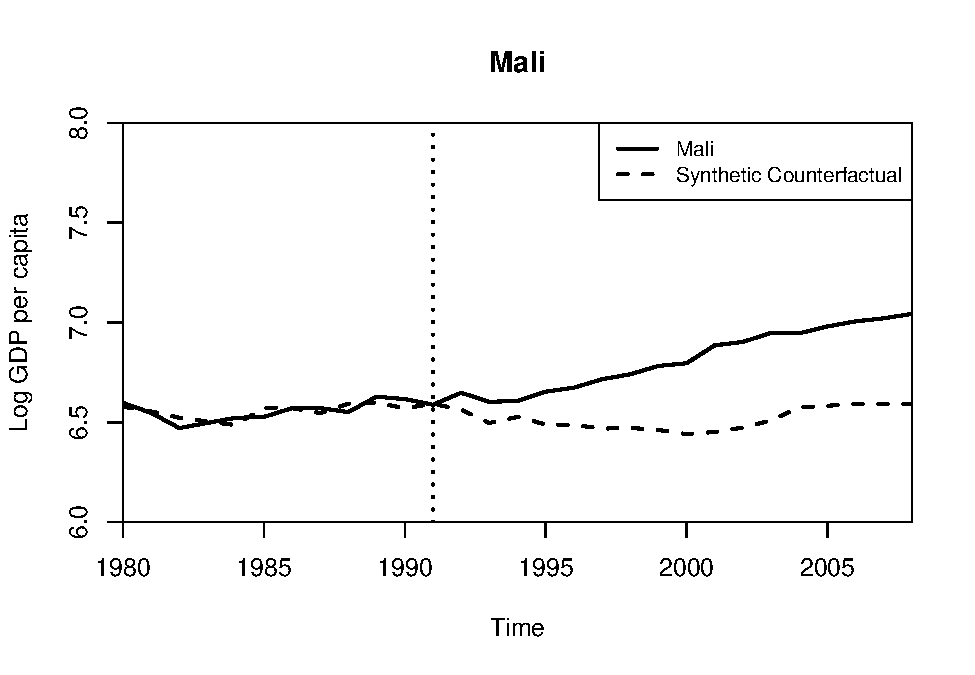
\includegraphics{ProjectNotebook_files/figure-latex/unnamed-chunk-4-1.pdf}

\begin{Shaded}
\begin{Highlighting}[]
\CommentTok{## Figure 2 Replication in-time placebo}
\KeywordTok{replicate}\NormalTok{(}\StringTok{"MLI"}\NormalTok{, }\StringTok{"Mali"}\NormalTok{, }\DecValTok{1980}\NormalTok{, }\DecValTok{1985}\NormalTok{, }\DecValTok{1986}\NormalTok{, }\DecValTok{2008}\NormalTok{, }\DecValTok{6}\NormalTok{, }\DecValTok{8}\NormalTok{)}
\end{Highlighting}
\end{Shaded}

\begin{verbatim}
## 
##  Missing data- treated unit; predictor: eximdiff_lag1 ; for period: 1980 
##  We ignore (na.rm = TRUE) all missing values for predictors.op.
## 
##  Missing data- treated unit; predictor: eximdiff_lag2 ; for period: 1980 
##  We ignore (na.rm = TRUE) all missing values for predictors.op.
## 
##  Missing data- treated unit; predictor: eximdiff_lag2 ; for period: 1981 
##  We ignore (na.rm = TRUE) all missing values for predictors.op.
## 
##  Missing data - control unit: 2 ; predictor: eximdiff_lag1 ; for period: 1980 
##  We ignore (na.rm = TRUE) all missing values for predictors.op.
## 
##  Missing data - control unit: 11 ; predictor: eximdiff_lag1 ; for period: 1980 
##  We ignore (na.rm = TRUE) all missing values for predictors.op.
## 
##  Missing data - control unit: 14 ; predictor: eximdiff_lag1 ; for period: 1980 
##  We ignore (na.rm = TRUE) all missing values for predictors.op.
## 
##  Missing data - control unit: 2 ; predictor: eximdiff_lag2 ; for period: 1980 
##  We ignore (na.rm = TRUE) all missing values for predictors.op.
## 
##  Missing data - control unit: 2 ; predictor: eximdiff_lag2 ; for period: 1981 
##  We ignore (na.rm = TRUE) all missing values for predictors.op.
## 
##  Missing data - control unit: 11 ; predictor: eximdiff_lag2 ; for period: 1980 
##  We ignore (na.rm = TRUE) all missing values for predictors.op.
## 
##  Missing data - control unit: 11 ; predictor: eximdiff_lag2 ; for period: 1981 
##  We ignore (na.rm = TRUE) all missing values for predictors.op.
## 
##  Missing data - control unit: 14 ; predictor: eximdiff_lag2 ; for period: 1980 
##  We ignore (na.rm = TRUE) all missing values for predictors.op.
## 
##  Missing data - control unit: 14 ; predictor: eximdiff_lag2 ; for period: 1981 
##  We ignore (na.rm = TRUE) all missing values for predictors.op.
## 
## X1, X0, Z1, Z0 all come directly from dataprep object.
## 
## 
## **************** 
##  searching for synthetic control unit  
##  
## 
## **************** 
## **************** 
## **************** 
## 
## MSPE (LOSS V): 0.00088 
## 
## solution.v:
##  0.138 0.177 0.158 0.132 0.0885 0.00037 0.153 0.00231 0.00662 0.0181 0.0163 0.0152 0.0195 0.00283 0.0087 0.0635 
## 
## solution.w:
##  0.00000594 0.221 0.00205 0.0000551 0.0000317 0.0000295 0.000000555 0.000000407 0.00000973 0.0000184 0.00423 0.173 0.000168 0.00000673 0.262 0.338 0.0000133
\end{verbatim}

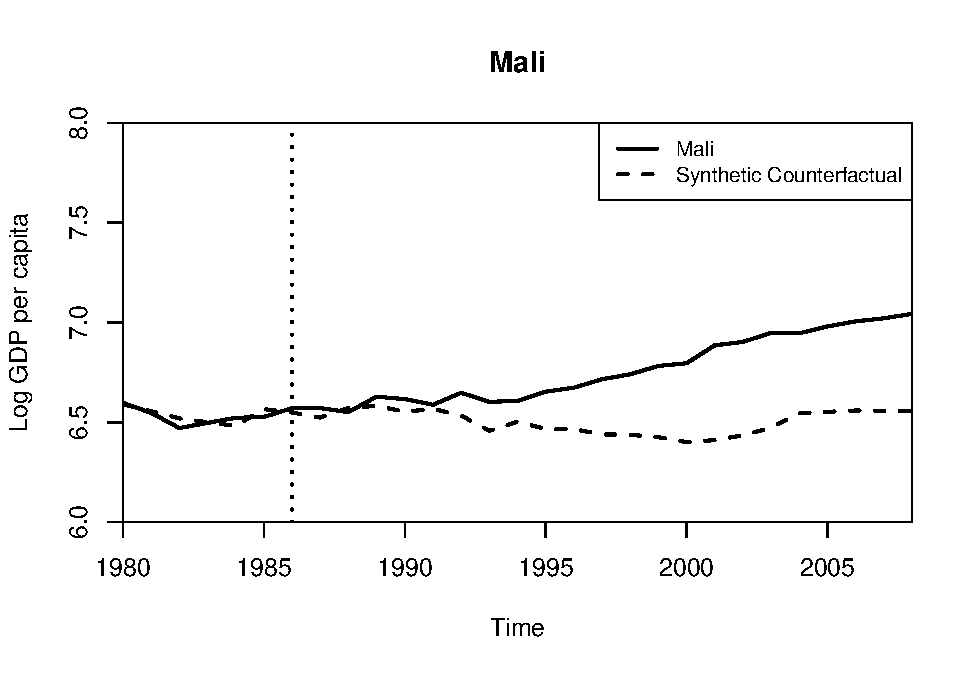
\includegraphics{ProjectNotebook_files/figure-latex/unnamed-chunk-5-1.pdf}

\begin{Shaded}
\begin{Highlighting}[]
\CommentTok{## Figure 2 Replication in-space placebo}
\KeywordTok{replicate}\NormalTok{(}\StringTok{"BFA"}\NormalTok{, }\StringTok{"Burkina Faso"}\NormalTok{, }\DecValTok{1980}\NormalTok{, }\DecValTok{1990}\NormalTok{, }\DecValTok{1991}\NormalTok{, }\DecValTok{2008}\NormalTok{, }\DecValTok{6}\NormalTok{, }\DecValTok{8}\NormalTok{)  }
\end{Highlighting}
\end{Shaded}

\begin{verbatim}
## 
##  Missing data- treated unit; predictor: eximdiff_lag1 ; for period: 1980 
##  We ignore (na.rm = TRUE) all missing values for predictors.op.
## 
##  Missing data- treated unit; predictor: eximdiff_lag2 ; for period: 1980 
##  We ignore (na.rm = TRUE) all missing values for predictors.op.
## 
##  Missing data- treated unit; predictor: eximdiff_lag2 ; for period: 1981 
##  We ignore (na.rm = TRUE) all missing values for predictors.op.
## 
##  Missing data - control unit: 2 ; predictor: eximdiff_lag1 ; for period: 1980 
##  We ignore (na.rm = TRUE) all missing values for predictors.op.
## 
##  Missing data - control unit: 11 ; predictor: eximdiff_lag1 ; for period: 1980 
##  We ignore (na.rm = TRUE) all missing values for predictors.op.
## 
##  Missing data - control unit: 2 ; predictor: eximdiff_lag2 ; for period: 1980 
##  We ignore (na.rm = TRUE) all missing values for predictors.op.
## 
##  Missing data - control unit: 2 ; predictor: eximdiff_lag2 ; for period: 1981 
##  We ignore (na.rm = TRUE) all missing values for predictors.op.
## 
##  Missing data - control unit: 11 ; predictor: eximdiff_lag2 ; for period: 1980 
##  We ignore (na.rm = TRUE) all missing values for predictors.op.
## 
##  Missing data - control unit: 11 ; predictor: eximdiff_lag2 ; for period: 1981 
##  We ignore (na.rm = TRUE) all missing values for predictors.op.
## 
## X1, X0, Z1, Z0 all come directly from dataprep object.
## 
## 
## **************** 
##  searching for synthetic control unit  
##  
## 
## **************** 
## **************** 
## **************** 
## 
## MSPE (LOSS V): 0.00204 
## 
## solution.v:
##  0.121 0.089 0.0518 0.0149 0.00506 0.389 0.015 0.00874 0.297 0.000311 0.00427 0.000802 0.00313 0.0000237 0.0000827 0.0000795 
## 
## solution.w:
##  0.00000702 0.179 0.0000307 0.0000148 0.0000224 0.0000146 0.000971 0.0000406 0.0000299 0.00674 0.000152 0.0000238 0.307 0.478 0.028 0.00000734
\end{verbatim}

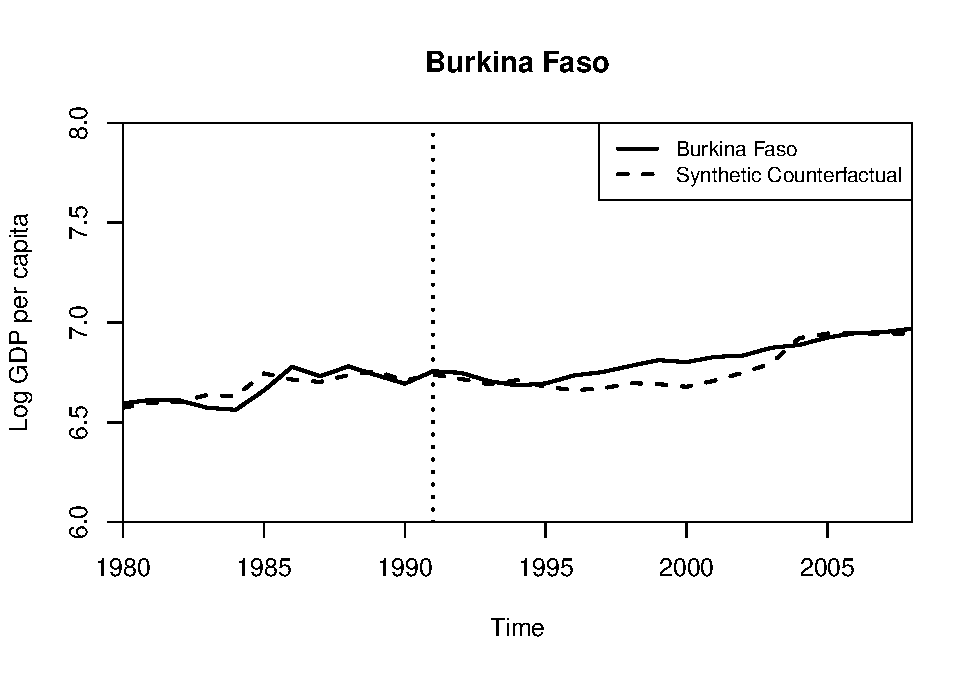
\includegraphics{ProjectNotebook_files/figure-latex/unnamed-chunk-6-1.pdf}

\begin{Shaded}
\begin{Highlighting}[]
\CommentTok{## Figure 2 Replication in-space placebo}
\KeywordTok{replicate}\NormalTok{(}\StringTok{"TCD"}\NormalTok{, }\StringTok{"Chad"}\NormalTok{, }\DecValTok{1980}\NormalTok{, }\DecValTok{1990}\NormalTok{, }\DecValTok{1991}\NormalTok{, }\DecValTok{2008}\NormalTok{, }\DecValTok{6}\NormalTok{, }\DecValTok{8}\NormalTok{)  }
\end{Highlighting}
\end{Shaded}

\begin{verbatim}
## 
##  Missing data- treated unit; predictor: eximdiff_lag1 ; for period: 1980 
##  We ignore (na.rm = TRUE) all missing values for predictors.op.
## 
##  Missing data- treated unit; predictor: eximdiff_lag2 ; for period: 1980 
##  We ignore (na.rm = TRUE) all missing values for predictors.op.
## 
##  Missing data- treated unit; predictor: eximdiff_lag2 ; for period: 1981 
##  We ignore (na.rm = TRUE) all missing values for predictors.op.
## 
##  Missing data - control unit: 2 ; predictor: eximdiff_lag1 ; for period: 1980 
##  We ignore (na.rm = TRUE) all missing values for predictors.op.
## 
##  Missing data - control unit: 11 ; predictor: eximdiff_lag1 ; for period: 1980 
##  We ignore (na.rm = TRUE) all missing values for predictors.op.
## 
##  Missing data - control unit: 2 ; predictor: eximdiff_lag2 ; for period: 1980 
##  We ignore (na.rm = TRUE) all missing values for predictors.op.
## 
##  Missing data - control unit: 2 ; predictor: eximdiff_lag2 ; for period: 1981 
##  We ignore (na.rm = TRUE) all missing values for predictors.op.
## 
##  Missing data - control unit: 11 ; predictor: eximdiff_lag2 ; for period: 1980 
##  We ignore (na.rm = TRUE) all missing values for predictors.op.
## 
##  Missing data - control unit: 11 ; predictor: eximdiff_lag2 ; for period: 1981 
##  We ignore (na.rm = TRUE) all missing values for predictors.op.
## 
## X1, X0, Z1, Z0 all come directly from dataprep object.
## 
## 
## **************** 
##  searching for synthetic control unit  
##  
## 
## **************** 
## **************** 
## **************** 
## 
## MSPE (LOSS V): 0.137 
## 
## solution.v:
##  0.195 0.196 0.185 0.163 0.00631 0.152 0.0817 0.000166 0.00515 0.00198 0.00066 0.00208 0.00693 0.00112 0.000519 0.00337 
## 
## solution.w:
##  0.0000000374 0.000000465 0.000000212 0.000000294 0.0000000066 0.0000000067 2e-10 0.0000000194 0.0000000366 0.0000000293 0.000000642 0.000000011 0.0000000628 0.0000000049 0.0000000974 1
\end{verbatim}

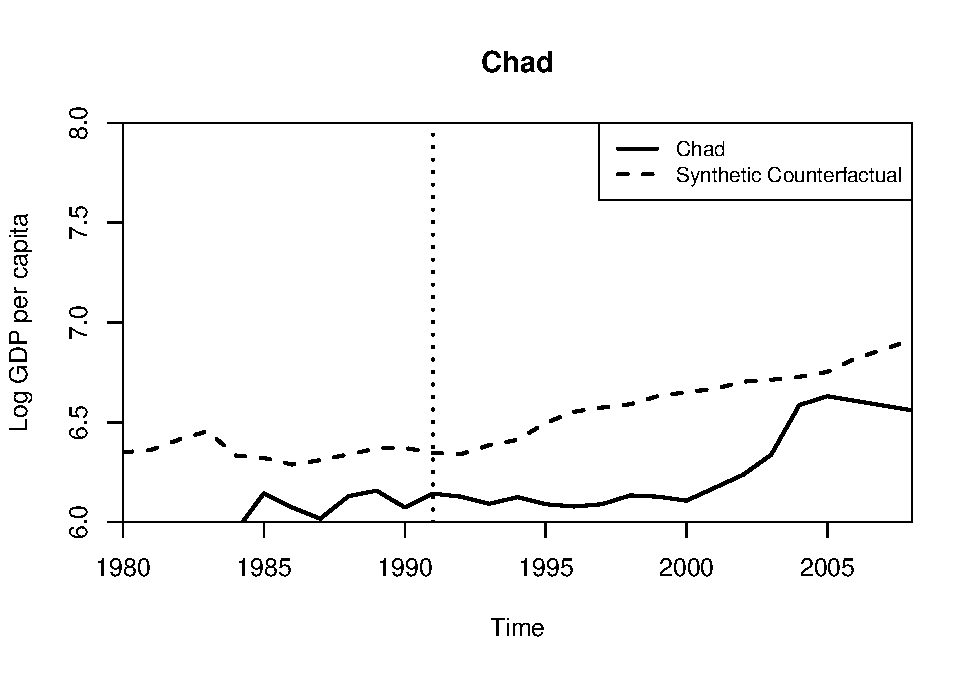
\includegraphics{ProjectNotebook_files/figure-latex/unnamed-chunk-7-1.pdf}

\begin{Shaded}
\begin{Highlighting}[]
\CommentTok{## Figure 2 Replication in-space placebo}
\KeywordTok{replicate}\NormalTok{(}\StringTok{"NGA"}\NormalTok{, }\StringTok{"Nigeria"}\NormalTok{, }\DecValTok{1980}\NormalTok{, }\DecValTok{1990}\NormalTok{, }\DecValTok{1991}\NormalTok{, }\DecValTok{2008}\NormalTok{, }\DecValTok{6}\NormalTok{, }\DecValTok{8}\NormalTok{)  }
\end{Highlighting}
\end{Shaded}

\begin{verbatim}
## 
##  Missing data- treated unit; predictor: eximdiff_lag1 ; for period: 1980 
##  We ignore (na.rm = TRUE) all missing values for predictors.op.
## 
##  Missing data- treated unit; predictor: eximdiff_lag2 ; for period: 1980 
##  We ignore (na.rm = TRUE) all missing values for predictors.op.
## 
##  Missing data- treated unit; predictor: eximdiff_lag2 ; for period: 1981 
##  We ignore (na.rm = TRUE) all missing values for predictors.op.
## 
##  Missing data - control unit: 2 ; predictor: eximdiff_lag1 ; for period: 1980 
##  We ignore (na.rm = TRUE) all missing values for predictors.op.
## 
##  Missing data - control unit: 11 ; predictor: eximdiff_lag1 ; for period: 1980 
##  We ignore (na.rm = TRUE) all missing values for predictors.op.
## 
##  Missing data - control unit: 2 ; predictor: eximdiff_lag2 ; for period: 1980 
##  We ignore (na.rm = TRUE) all missing values for predictors.op.
## 
##  Missing data - control unit: 2 ; predictor: eximdiff_lag2 ; for period: 1981 
##  We ignore (na.rm = TRUE) all missing values for predictors.op.
## 
##  Missing data - control unit: 11 ; predictor: eximdiff_lag2 ; for period: 1980 
##  We ignore (na.rm = TRUE) all missing values for predictors.op.
## 
##  Missing data - control unit: 11 ; predictor: eximdiff_lag2 ; for period: 1981 
##  We ignore (na.rm = TRUE) all missing values for predictors.op.
## 
## X1, X0, Z1, Z0 all come directly from dataprep object.
## 
## 
## **************** 
##  searching for synthetic control unit  
##  
## 
## **************** 
## **************** 
## **************** 
## 
## MSPE (LOSS V): 0.00607 
## 
## solution.v:
##  0.000759 0.00277 0.00137 0.000229 0.000000116 0.000000127 0.000000245 0.0000000019 0.000000124 0.0134 0.098 0.66 0.223 0.0000167 0.00012 0.0000575 
## 
## solution.w:
##  0.137 0.0182 0.0172 0.0183 0.019 0.0138 0.137 0.467 0.024 0.0192 0.018 0.0182 0.00818 0.0176 0.0183 0.0483
\end{verbatim}

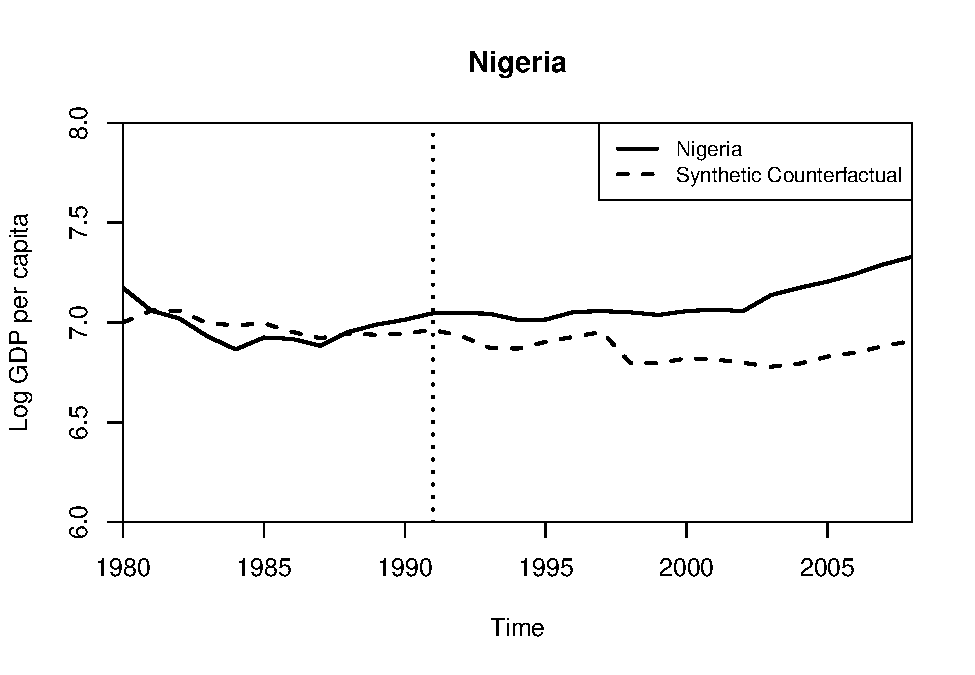
\includegraphics{ProjectNotebook_files/figure-latex/unnamed-chunk-8-1.pdf}

\begin{Shaded}
\begin{Highlighting}[]
\CommentTok{## Figure 2 Replication in-space placebo}
\KeywordTok{replicate}\NormalTok{(}\StringTok{"BDI"}\NormalTok{, }\StringTok{"Burundi"}\NormalTok{, }\DecValTok{1980}\NormalTok{, }\DecValTok{1990}\NormalTok{, }\DecValTok{1991}\NormalTok{, }\DecValTok{2008}\NormalTok{, }\DecValTok{6}\NormalTok{, }\DecValTok{8}\NormalTok{)  }
\end{Highlighting}
\end{Shaded}

\begin{verbatim}
## 
##  Missing data- treated unit; predictor: eximdiff_lag1 ; for period: 1980 
##  We ignore (na.rm = TRUE) all missing values for predictors.op.
## 
##  Missing data- treated unit; predictor: eximdiff_lag2 ; for period: 1980 
##  We ignore (na.rm = TRUE) all missing values for predictors.op.
## 
##  Missing data- treated unit; predictor: eximdiff_lag2 ; for period: 1981 
##  We ignore (na.rm = TRUE) all missing values for predictors.op.
## 
##  Missing data - control unit: 2 ; predictor: eximdiff_lag1 ; for period: 1980 
##  We ignore (na.rm = TRUE) all missing values for predictors.op.
## 
##  Missing data - control unit: 14 ; predictor: eximdiff_lag1 ; for period: 1980 
##  We ignore (na.rm = TRUE) all missing values for predictors.op.
## 
##  Missing data - control unit: 2 ; predictor: eximdiff_lag2 ; for period: 1980 
##  We ignore (na.rm = TRUE) all missing values for predictors.op.
## 
##  Missing data - control unit: 2 ; predictor: eximdiff_lag2 ; for period: 1981 
##  We ignore (na.rm = TRUE) all missing values for predictors.op.
## 
##  Missing data - control unit: 14 ; predictor: eximdiff_lag2 ; for period: 1980 
##  We ignore (na.rm = TRUE) all missing values for predictors.op.
## 
##  Missing data - control unit: 14 ; predictor: eximdiff_lag2 ; for period: 1981 
##  We ignore (na.rm = TRUE) all missing values for predictors.op.
## 
## X1, X0, Z1, Z0 all come directly from dataprep object.
## 
## 
## **************** 
##  searching for synthetic control unit  
##  
## 
## **************** 
## **************** 
## **************** 
## 
## MSPE (LOSS V): 0.00101 
## 
## solution.v:
##  0.0105 0.00107 0.000214 0.000229 0.0176 0.0309 0.0000000896 0.000000582 0.000000266 0.0141 0.0919 0.618 0.213 0.00267 0.000375 0.0000147 
## 
## solution.w:
##  0.00137 0.157 0.000636 0.00174 0.108 0.00158 0.115 0.00143 0.00186 0.026 0.0706 0.00207 0.00212 0.507 0.00296 0.00123
\end{verbatim}

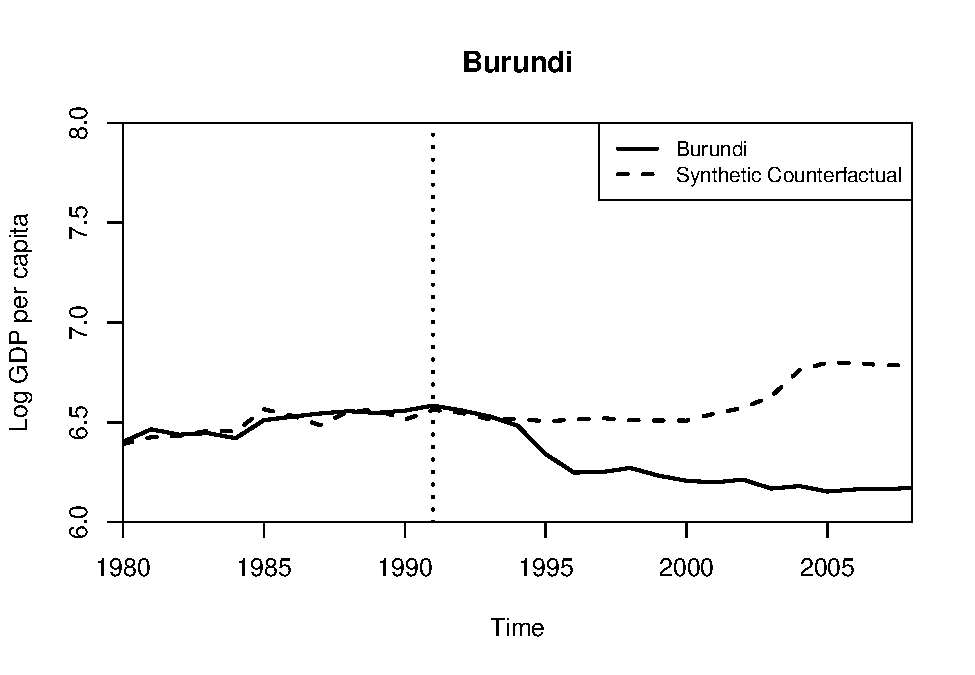
\includegraphics{ProjectNotebook_files/figure-latex/unnamed-chunk-9-1.pdf}

\begin{Shaded}
\begin{Highlighting}[]
\CommentTok{## Figure 2 Replication in-space placebo}
\KeywordTok{replicate}\NormalTok{(}\StringTok{"TGO"}\NormalTok{, }\StringTok{"Togo"}\NormalTok{, }\DecValTok{1980}\NormalTok{, }\DecValTok{1990}\NormalTok{, }\DecValTok{1991}\NormalTok{, }\DecValTok{2008}\NormalTok{, }\DecValTok{6}\NormalTok{, }\DecValTok{8}\NormalTok{)  }
\end{Highlighting}
\end{Shaded}

\begin{verbatim}
## 
##  Missing data- treated unit; predictor: eximdiff_lag1 ; for period: 1980 
##  We ignore (na.rm = TRUE) all missing values for predictors.op.
## 
##  Missing data- treated unit; predictor: eximdiff_lag2 ; for period: 1980 
##  We ignore (na.rm = TRUE) all missing values for predictors.op.
## 
##  Missing data- treated unit; predictor: eximdiff_lag2 ; for period: 1981 
##  We ignore (na.rm = TRUE) all missing values for predictors.op.
## 
##  Missing data - control unit: 2 ; predictor: eximdiff_lag1 ; for period: 1980 
##  We ignore (na.rm = TRUE) all missing values for predictors.op.
## 
##  Missing data - control unit: 11 ; predictor: eximdiff_lag1 ; for period: 1980 
##  We ignore (na.rm = TRUE) all missing values for predictors.op.
## 
##  Missing data - control unit: 2 ; predictor: eximdiff_lag2 ; for period: 1980 
##  We ignore (na.rm = TRUE) all missing values for predictors.op.
## 
##  Missing data - control unit: 2 ; predictor: eximdiff_lag2 ; for period: 1981 
##  We ignore (na.rm = TRUE) all missing values for predictors.op.
## 
##  Missing data - control unit: 11 ; predictor: eximdiff_lag2 ; for period: 1980 
##  We ignore (na.rm = TRUE) all missing values for predictors.op.
## 
##  Missing data - control unit: 11 ; predictor: eximdiff_lag2 ; for period: 1981 
##  We ignore (na.rm = TRUE) all missing values for predictors.op.
## 
## X1, X0, Z1, Z0 all come directly from dataprep object.
## 
## 
## **************** 
##  searching for synthetic control unit  
##  
## 
## **************** 
## **************** 
## **************** 
## 
## MSPE (LOSS V): 0.00313 
## 
## solution.v:
##  0.0239 0.00267 0.00904 0.00021 0.000000499 0.00000214 0.000000173 0.031 0.000000331 0.0126 0.0919 0.619 0.209 0.00000176 0.0000635 0.00000155 
## 
## solution.w:
##  0.000138 0.000551 0.0000373 0.0000122 0.245 0.00972 0.0536 0.000294 0.000279 0.000449 0.578 0.00028 0.000507 0.000267 0.11 0.000304
\end{verbatim}

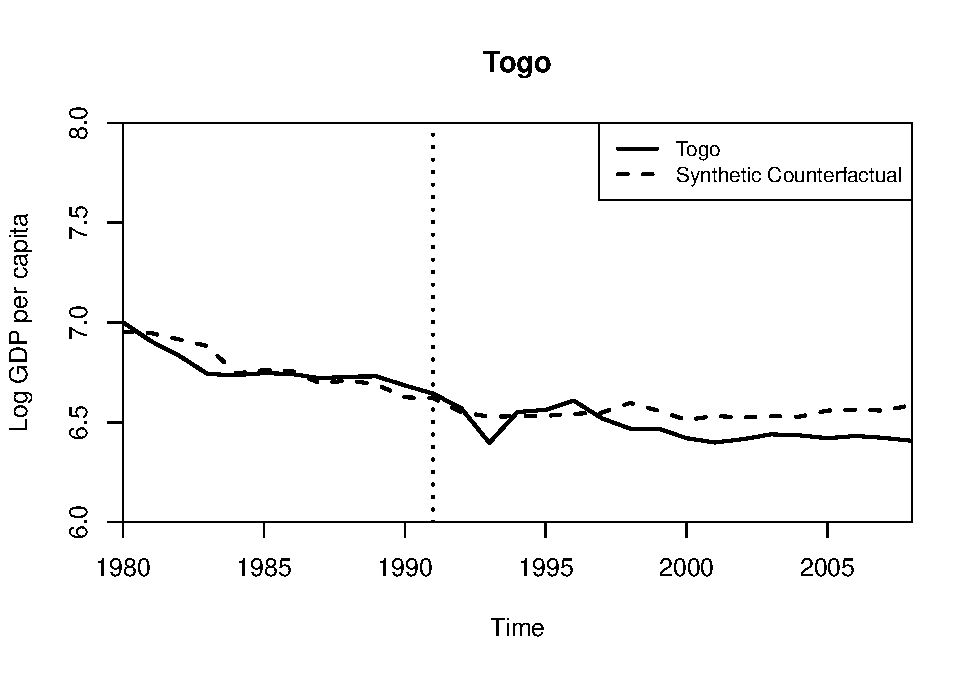
\includegraphics{ProjectNotebook_files/figure-latex/unnamed-chunk-10-1.pdf}

\hypertarget{extensions}{%
\subsection{Extensions}\label{extensions}}

\hypertarget{google-extension-causalimpact}{%
\subsubsection{Google Extension
(CausalImpact)}\label{google-extension-causalimpact}}

\begin{Shaded}
\begin{Highlighting}[]
\CommentTok{# Replication function from Google Extension}
\NormalTok{show_impact_n <-}\StringTok{ }\ControlFlowTok{function}\NormalTok{(}
\NormalTok{  Country,}
\NormalTok{  begin,}
\NormalTok{  end,}
\NormalTok{  treatYear}
\NormalTok{)\{}
\NormalTok{  data <-}\StringTok{ }\NormalTok{afripanel[}\KeywordTok{which}\NormalTok{(afripanel}\OperatorTok{$}\NormalTok{Country }\OperatorTok{==}\StringTok{ }\NormalTok{Country), ]}
\NormalTok{  predictors=}\KeywordTok{c}\NormalTok{(}
      \StringTok{"lngdpmadlag"}\NormalTok{,}
      \StringTok{"lngdpmadlag2"}\NormalTok{,}
      \StringTok{"lngdpmadlag3"}\NormalTok{,}
      \StringTok{"lngdpmadlag4"}\NormalTok{,}
      \StringTok{"lnpop"}\NormalTok{,}
      \StringTok{"ki"}\NormalTok{,}
      \StringTok{"openk"}\NormalTok{,}
      \StringTok{"civwar"}\NormalTok{,}
      \StringTok{"civwarend"}\NormalTok{,}
      \StringTok{"pwt_xrate"}\NormalTok{,}
      \StringTok{"pwt_xrate_lag1"}\NormalTok{,}
      \StringTok{"pwt_xrate_lag2"}\NormalTok{,}
      \StringTok{"pwt_xrate_lag3"}\NormalTok{,}
      \StringTok{"eximdiff"}\NormalTok{,}
      \StringTok{"eximdiff_lag1"}\NormalTok{,}
      \StringTok{"eximdiff_lag2"}\NormalTok{,}
      \StringTok{"wbank"}\NormalTok{,}
      \StringTok{"wbank_lag1"}\NormalTok{,}
      \StringTok{"wbank_lag2"}
\NormalTok{  )}

\NormalTok{  outcome <-}\StringTok{ 'lngdpmad'}
\NormalTok{  time.points <-}\StringTok{ }\KeywordTok{as.Date}\NormalTok{(}\KeywordTok{as.character}\NormalTok{(data}\OperatorTok{$}\NormalTok{year), }\StringTok{"%Y"}\NormalTok{)}
  
\NormalTok{  data <-}\StringTok{ }\NormalTok{data[, }\KeywordTok{c}\NormalTok{(outcome, predictors)]}
\NormalTok{  data<-data[}\OperatorTok{!}\KeywordTok{is.na}\NormalTok{(data[outcome]),]}
\NormalTok{  data <-}\StringTok{ }\NormalTok{data }\OperatorTok\StringTok{ }\KeywordTok{select_if}\NormalTok{(not_any_na)}
  
  
\NormalTok{  data <-}\StringTok{ }\KeywordTok{zoo}\NormalTok{(data, time.points)}
\NormalTok{  data <-}\StringTok{ }\NormalTok{data[}\KeywordTok{index}\NormalTok{(data) }\OperatorTok{>}\StringTok{ }\KeywordTok{as.Date}\NormalTok{(begin, }\StringTok{'%Y'}\NormalTok{) }\OperatorTok{&}\StringTok{ }\KeywordTok{index}\NormalTok{(data) }\OperatorTok{<}\StringTok{ }\KeywordTok{as.Date}\NormalTok{(end, }\StringTok{'%Y'}\NormalTok{)]}
  
\NormalTok{  nextYear <-}\StringTok{ }\KeywordTok{as.Date}\NormalTok{(}\KeywordTok{as.character}\NormalTok{(}\KeywordTok{as.numeric}\NormalTok{(treatYear) }\OperatorTok{+}\StringTok{ }\DecValTok{1}\NormalTok{), }\StringTok{"%Y"}\NormalTok{)}
\NormalTok{  treatYear <-}\StringTok{ }\KeywordTok{as.Date}\NormalTok{(treatYear, }\StringTok{"%Y"}\NormalTok{)}
  
\NormalTok{  start_date <-}\StringTok{ }\KeywordTok{start}\NormalTok{(data)}
\NormalTok{  end_date <-}\StringTok{ }\KeywordTok{end}\NormalTok{(data)}
  
\NormalTok{  pre.period <-}\StringTok{ }\KeywordTok{as.Date}\NormalTok{(}\KeywordTok{c}\NormalTok{(start_date, treatYear))}
\NormalTok{  post.period <-}\StringTok{ }\KeywordTok{as.Date}\NormalTok{(}\KeywordTok{c}\NormalTok{(nextYear, end_date))}
  
\NormalTok{  impact <-}\StringTok{ }\KeywordTok{CausalImpact}\NormalTok{(data, }
\NormalTok{                          pre.period, }
\NormalTok{                          post.period,}
                          \DataTypeTok{model.args =} \KeywordTok{list}\NormalTok{(}
                            \DataTypeTok{niter =} \DecValTok{1000}\NormalTok{, }
                            \DataTypeTok{nseasons =} \DecValTok{52}\NormalTok{)}
\NormalTok{                          )}
  \KeywordTok{return}\NormalTok{(impact)}
\NormalTok{\}}
\end{Highlighting}
\end{Shaded}

\hypertarget{graphs}{%
\section{Graphs:}\label{graphs}}

\begin{Shaded}
\begin{Highlighting}[]
\NormalTok{impact <-}\StringTok{ }\KeywordTok{show_impact_n}\NormalTok{(}\StringTok{'Mali'}\NormalTok{, }\StringTok{'1980'}\NormalTok{, }\StringTok{'2005'}\NormalTok{, }\StringTok{'1990'}\NormalTok{)}
\KeywordTok{plot}\NormalTok{(impact) }\OperatorTok{+}\StringTok{ }\KeywordTok{ggtitle}\NormalTok{ (}\StringTok{"Causal Impact on Mali beyond 1991"}\NormalTok{)}
\end{Highlighting}
\end{Shaded}

\begin{verbatim}
## Warning: Removed 24 rows containing missing values (geom_path).
\end{verbatim}

\begin{verbatim}
## Warning: Removed 48 rows containing missing values (geom_path).
\end{verbatim}

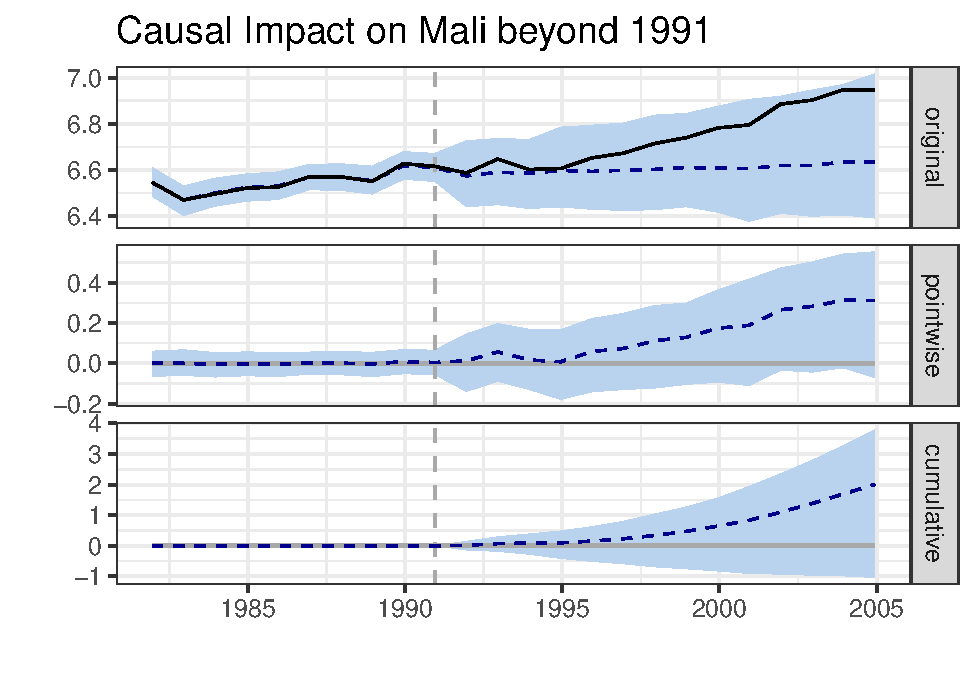
\includegraphics{ProjectNotebook_files/figure-latex/unnamed-chunk-12-1.pdf}

\begin{Shaded}
\begin{Highlighting}[]
\NormalTok{impact <-}\StringTok{ }\KeywordTok{show_impact_n}\NormalTok{(}\StringTok{'Mali'}\NormalTok{, }\StringTok{'1980'}\NormalTok{, }\StringTok{'2005'}\NormalTok{, }\StringTok{'1985'}\NormalTok{)}
\KeywordTok{plot}\NormalTok{(impact) }\OperatorTok{+}\StringTok{ }\KeywordTok{ggtitle}\NormalTok{(}\StringTok{"Causal Impact on Mali beyond 1985"}\NormalTok{)}
\end{Highlighting}
\end{Shaded}

\begin{verbatim}
## Warning: Removed 24 rows containing missing values (geom_path).
\end{verbatim}

\begin{verbatim}
## Warning: Removed 48 rows containing missing values (geom_path).
\end{verbatim}

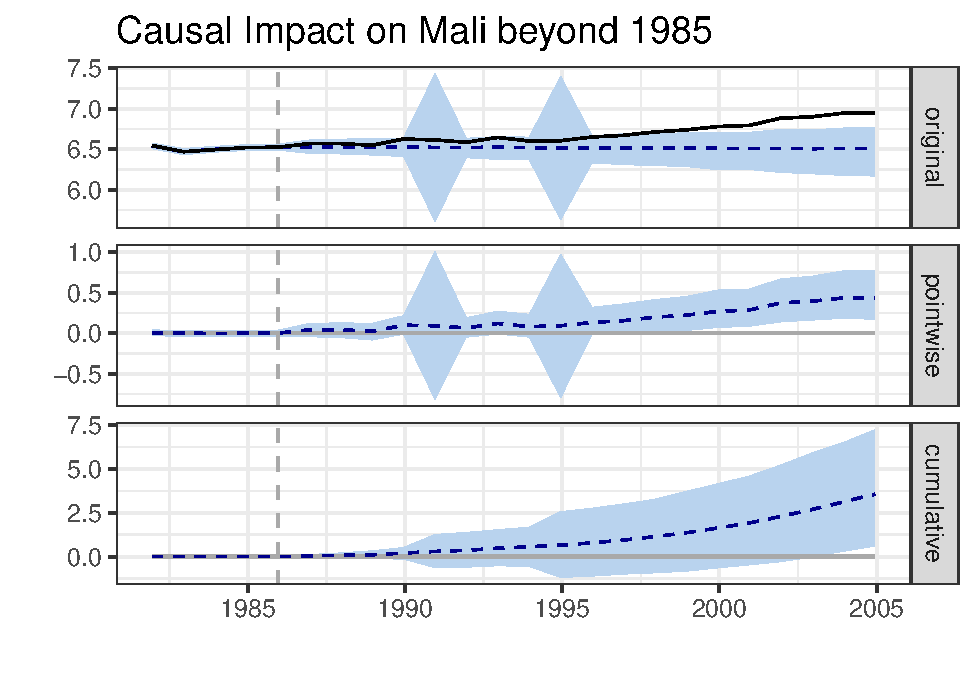
\includegraphics{ProjectNotebook_files/figure-latex/unnamed-chunk-13-1.pdf}

\begin{Shaded}
\begin{Highlighting}[]
\NormalTok{impact <-}\StringTok{ }\KeywordTok{show_impact_n}\NormalTok{(}\StringTok{'Burkina Faso'}\NormalTok{, }\StringTok{'1980'}\NormalTok{, }\StringTok{'2005'}\NormalTok{, }\StringTok{'1990'}\NormalTok{)}
\KeywordTok{plot}\NormalTok{(impact) }\OperatorTok{+}\StringTok{ }\KeywordTok{ggtitle}\NormalTok{(}\StringTok{"Causal Impact on Burkina Faso beyond 1990"}\NormalTok{)}
\end{Highlighting}
\end{Shaded}

\begin{verbatim}
## Warning: Removed 24 rows containing missing values (geom_path).
\end{verbatim}

\begin{verbatim}
## Warning: Removed 48 rows containing missing values (geom_path).
\end{verbatim}

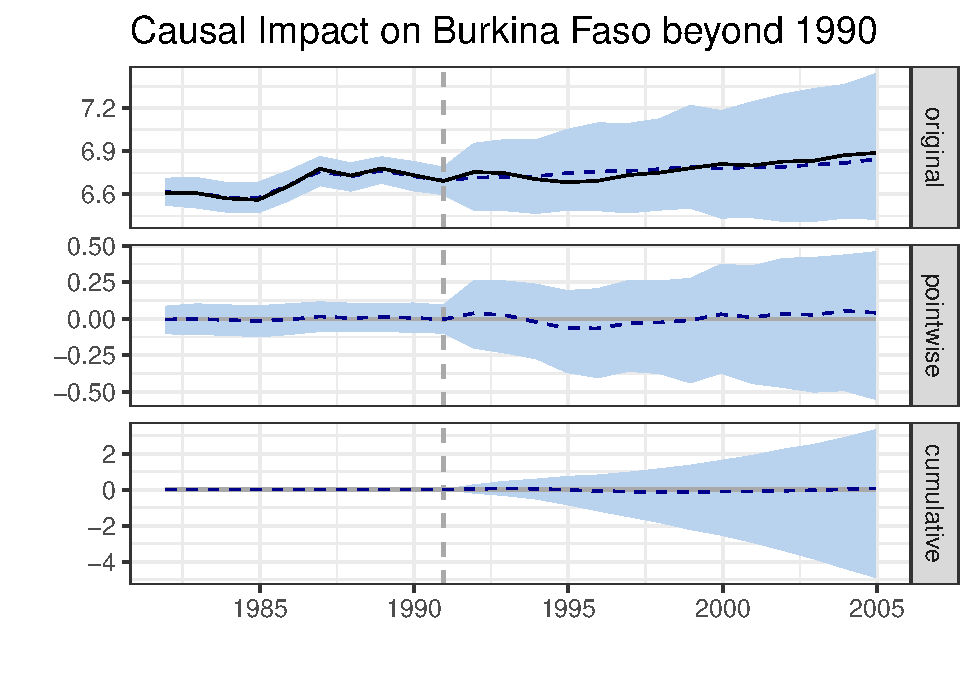
\includegraphics{ProjectNotebook_files/figure-latex/unnamed-chunk-14-1.pdf}

\begin{Shaded}
\begin{Highlighting}[]
\NormalTok{impact <-}\StringTok{ }\KeywordTok{show_impact_n}\NormalTok{(}\StringTok{'Mali'}\NormalTok{, }\StringTok{'1980'}\NormalTok{, }\StringTok{'2005'}\NormalTok{, }\StringTok{'1985'}\NormalTok{)}
\KeywordTok{plot}\NormalTok{(impact) }\OperatorTok{+}\StringTok{ }\KeywordTok{ggtitle}\NormalTok{(}\StringTok{"In-time placebo (Mali)"}\NormalTok{)}
\end{Highlighting}
\end{Shaded}

\begin{verbatim}
## Warning: Removed 24 rows containing missing values (geom_path).
\end{verbatim}

\begin{verbatim}
## Warning: Removed 48 rows containing missing values (geom_path).
\end{verbatim}

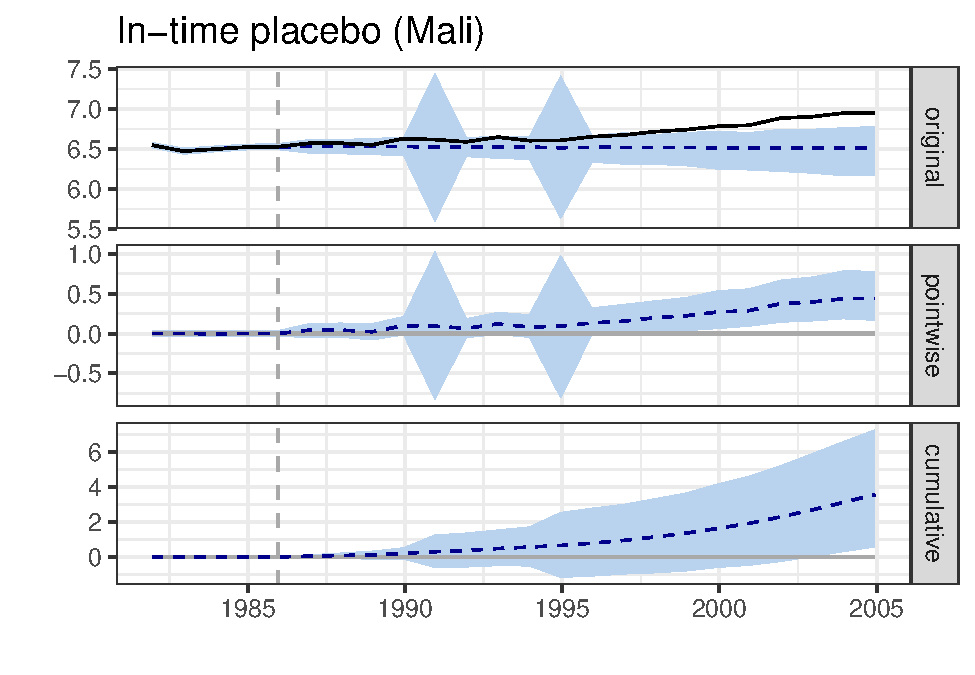
\includegraphics{ProjectNotebook_files/figure-latex/unnamed-chunk-15-1.pdf}

\begin{Shaded}
\begin{Highlighting}[]
\NormalTok{impact <-}\StringTok{ }\KeywordTok{show_impact_n}\NormalTok{(}\StringTok{'Burkina Faso'}\NormalTok{, }\StringTok{'1980'}\NormalTok{, }\StringTok{'2005'}\NormalTok{, }\StringTok{'1990'}\NormalTok{)}
\KeywordTok{plot}\NormalTok{(impact) }\OperatorTok{+}\StringTok{ }\KeywordTok{ggtitle}\NormalTok{(}\StringTok{"In-space placebo (Burkina Faso)"}\NormalTok{)}
\end{Highlighting}
\end{Shaded}

\begin{verbatim}
## Warning: Removed 24 rows containing missing values (geom_path).
\end{verbatim}

\begin{verbatim}
## Warning: Removed 48 rows containing missing values (geom_path).
\end{verbatim}

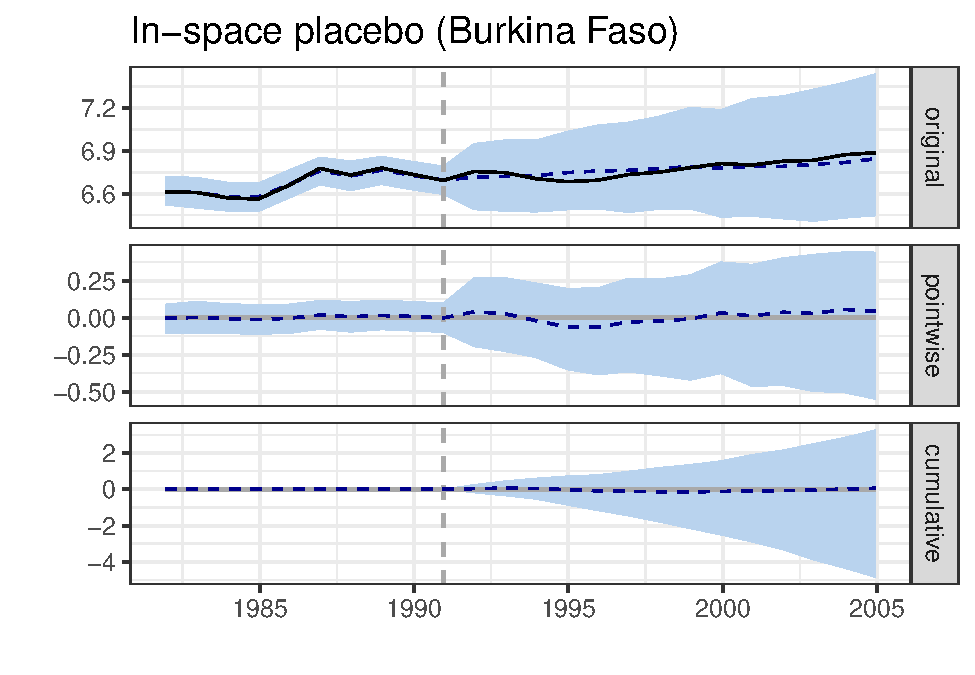
\includegraphics{ProjectNotebook_files/figure-latex/unnamed-chunk-16-1.pdf}


\end{document}
